\chapter{Act I: Robust End-to-End Driving via Test-Time Training}\label{ch:centaur}
\begin{contribution}
This chapter is based on the preprint ``Centaur: Robust End-to-End Autonomous Driving with Test-Time Training''~\cite{sima2024centaur}, of which the author is an equal-contribution first author with Kashyap Chitta and the primary contact. The work was carried out during the author's internship at NVIDIA Autonomous Vehicle Applied Research. The author proposed applying test-time training to end-to-end planning; designed Cluster Entropy; implemented Centaur on Hydra-MDP and conducted the NAVSIM experiments; designed and built the \texttt{navsafe} benchmark, including the scenario selection and its human verification; and conducted the analyses of failure detection, the ablations and the visualisations. The writing of the paper was led by co-authors.
\end{contribution}

Chapters~\ref{ch:occnet} and~\ref{ch:drivelm} addressed the first two stages of the perceive--reason--act loop: a general 3D representation and structured driving reasoning. The final and most direct test of a physical agent, however, is acting. The trajectory produced by an end-to-end planner is executed on a public road, so any error in it becomes a potential safety incident. This is also where the curse of reality is felt most acutely. However large its training set, a deployed vehicle keeps meeting rare, safety-critical situations that it has not seen during training, such as an unfamiliar roundabout, a yellow light that forces a choice between rushing and waiting, or a pedestrian who must be yielded to. This problem has been described as the curse of rarity for autonomous vehicles~\cite{liu2024curse}.

In current practice, a learned planner may be combined with a fallback layer that checks feasibility or with test-time trajectory optimisation using an explicit cost function. These safeguards have different information and engineering requirements. This chapter studies a complementary question for RQ3a: can a trajectory-scoring planner adapt its own parameters at test time using an uncertainty objective, without querying new expert labels or evaluating a new scene-dependent safety cost? The experiments compare this approach with a restricted fixed-trajectory fallback baseline; they do not establish that adaptation replaces safety filters in general.

This chapter answers the question with \emph{Centaur} (\textbf{C}luster \textbf{En}tropy for \textbf{T}est-time tr\textbf{A}ining using \textbf{U}nce\textbf{r}tainty), which updates a deployed planner through test-time training (TTT). It uses a gradient derived from recent frames and can compute that gradient asynchronously with inference. The chapter makes three contributions. First, it provides evidence that test-time training can improve a trajectory-scoring planner on the evaluated NAVSIM protocol. Second, it introduces Cluster Entropy, a direction-cluster score-mass objective whose structure makes alternative steering modes visible, while remaining sensitive to cluster cardinality. Third, it releases \texttt{navsafe}, a diagnostic stress set of 229 frames in ten NHTSA-inspired categories~\cite{najm2007pre}. All results use NAVSIM's non-reactive simulation~\cite{dauner2024navsim}. In a single v1.0 \texttt{navtest} run, Centaur changes Hydra-MDP's PDMS from 90.3 to 92.6, against 94.8 for logged human trajectories. Its three-seed NAVSIM v1.1 mean is 92.10 $\pm$ 0.33, first among three-seed entries at the paper's submission in March 2025. On \texttt{navsafe}, it has the highest displayed score in seven of ten categories but regresses on yielding; the source Overall aggregation is unresolved.

The chapter also builds on its predecessors. NAVSIM builds upon data from OpenScene~\cite{sima2023openscene}, described in Chapter~\ref{ch:occnet}, and nuPlan~\cite{caesar2021nuplan}, and the five direction anchors used by Cluster Entropy follow DriveLM~\cite{sima2024drivelm} (Chapter~\ref{ch:drivelm}).

The remainder of the chapter is organised as follows. Section~\ref{centaur:sec:intro} explains why today's safeguards are insufficient and why defining the uncertainty of a planner is non-trivial. Section~\ref{centaur:sec:related} reviews related work. Section~\ref{centaur:sec:method} presents Centaur, including Cluster Entropy and the test-time training procedure. Section~\ref{centaur:sec:navsafe} introduces the \texttt{navsafe} benchmark. Section~\ref{centaur:sec:exp} reports results on \texttt{navtest} and \texttt{navsafe}, and Section~\ref{centaur:sec:analysis} analyses qualitative behaviour, generality, design choices and computational cost. Section~\ref{centaur:sec:discussion} discusses the findings and their limitations, and Section~\ref{centaur:sec:summary} summarises the chapter. Additional related work, methodological details and ablations are given in Appendix~\ref{app:centaur}.

%-------------------------------------------------------------------------------
\section{Motivation}\label{centaur:sec:intro}

\begin{figure}[t]
  \centering
  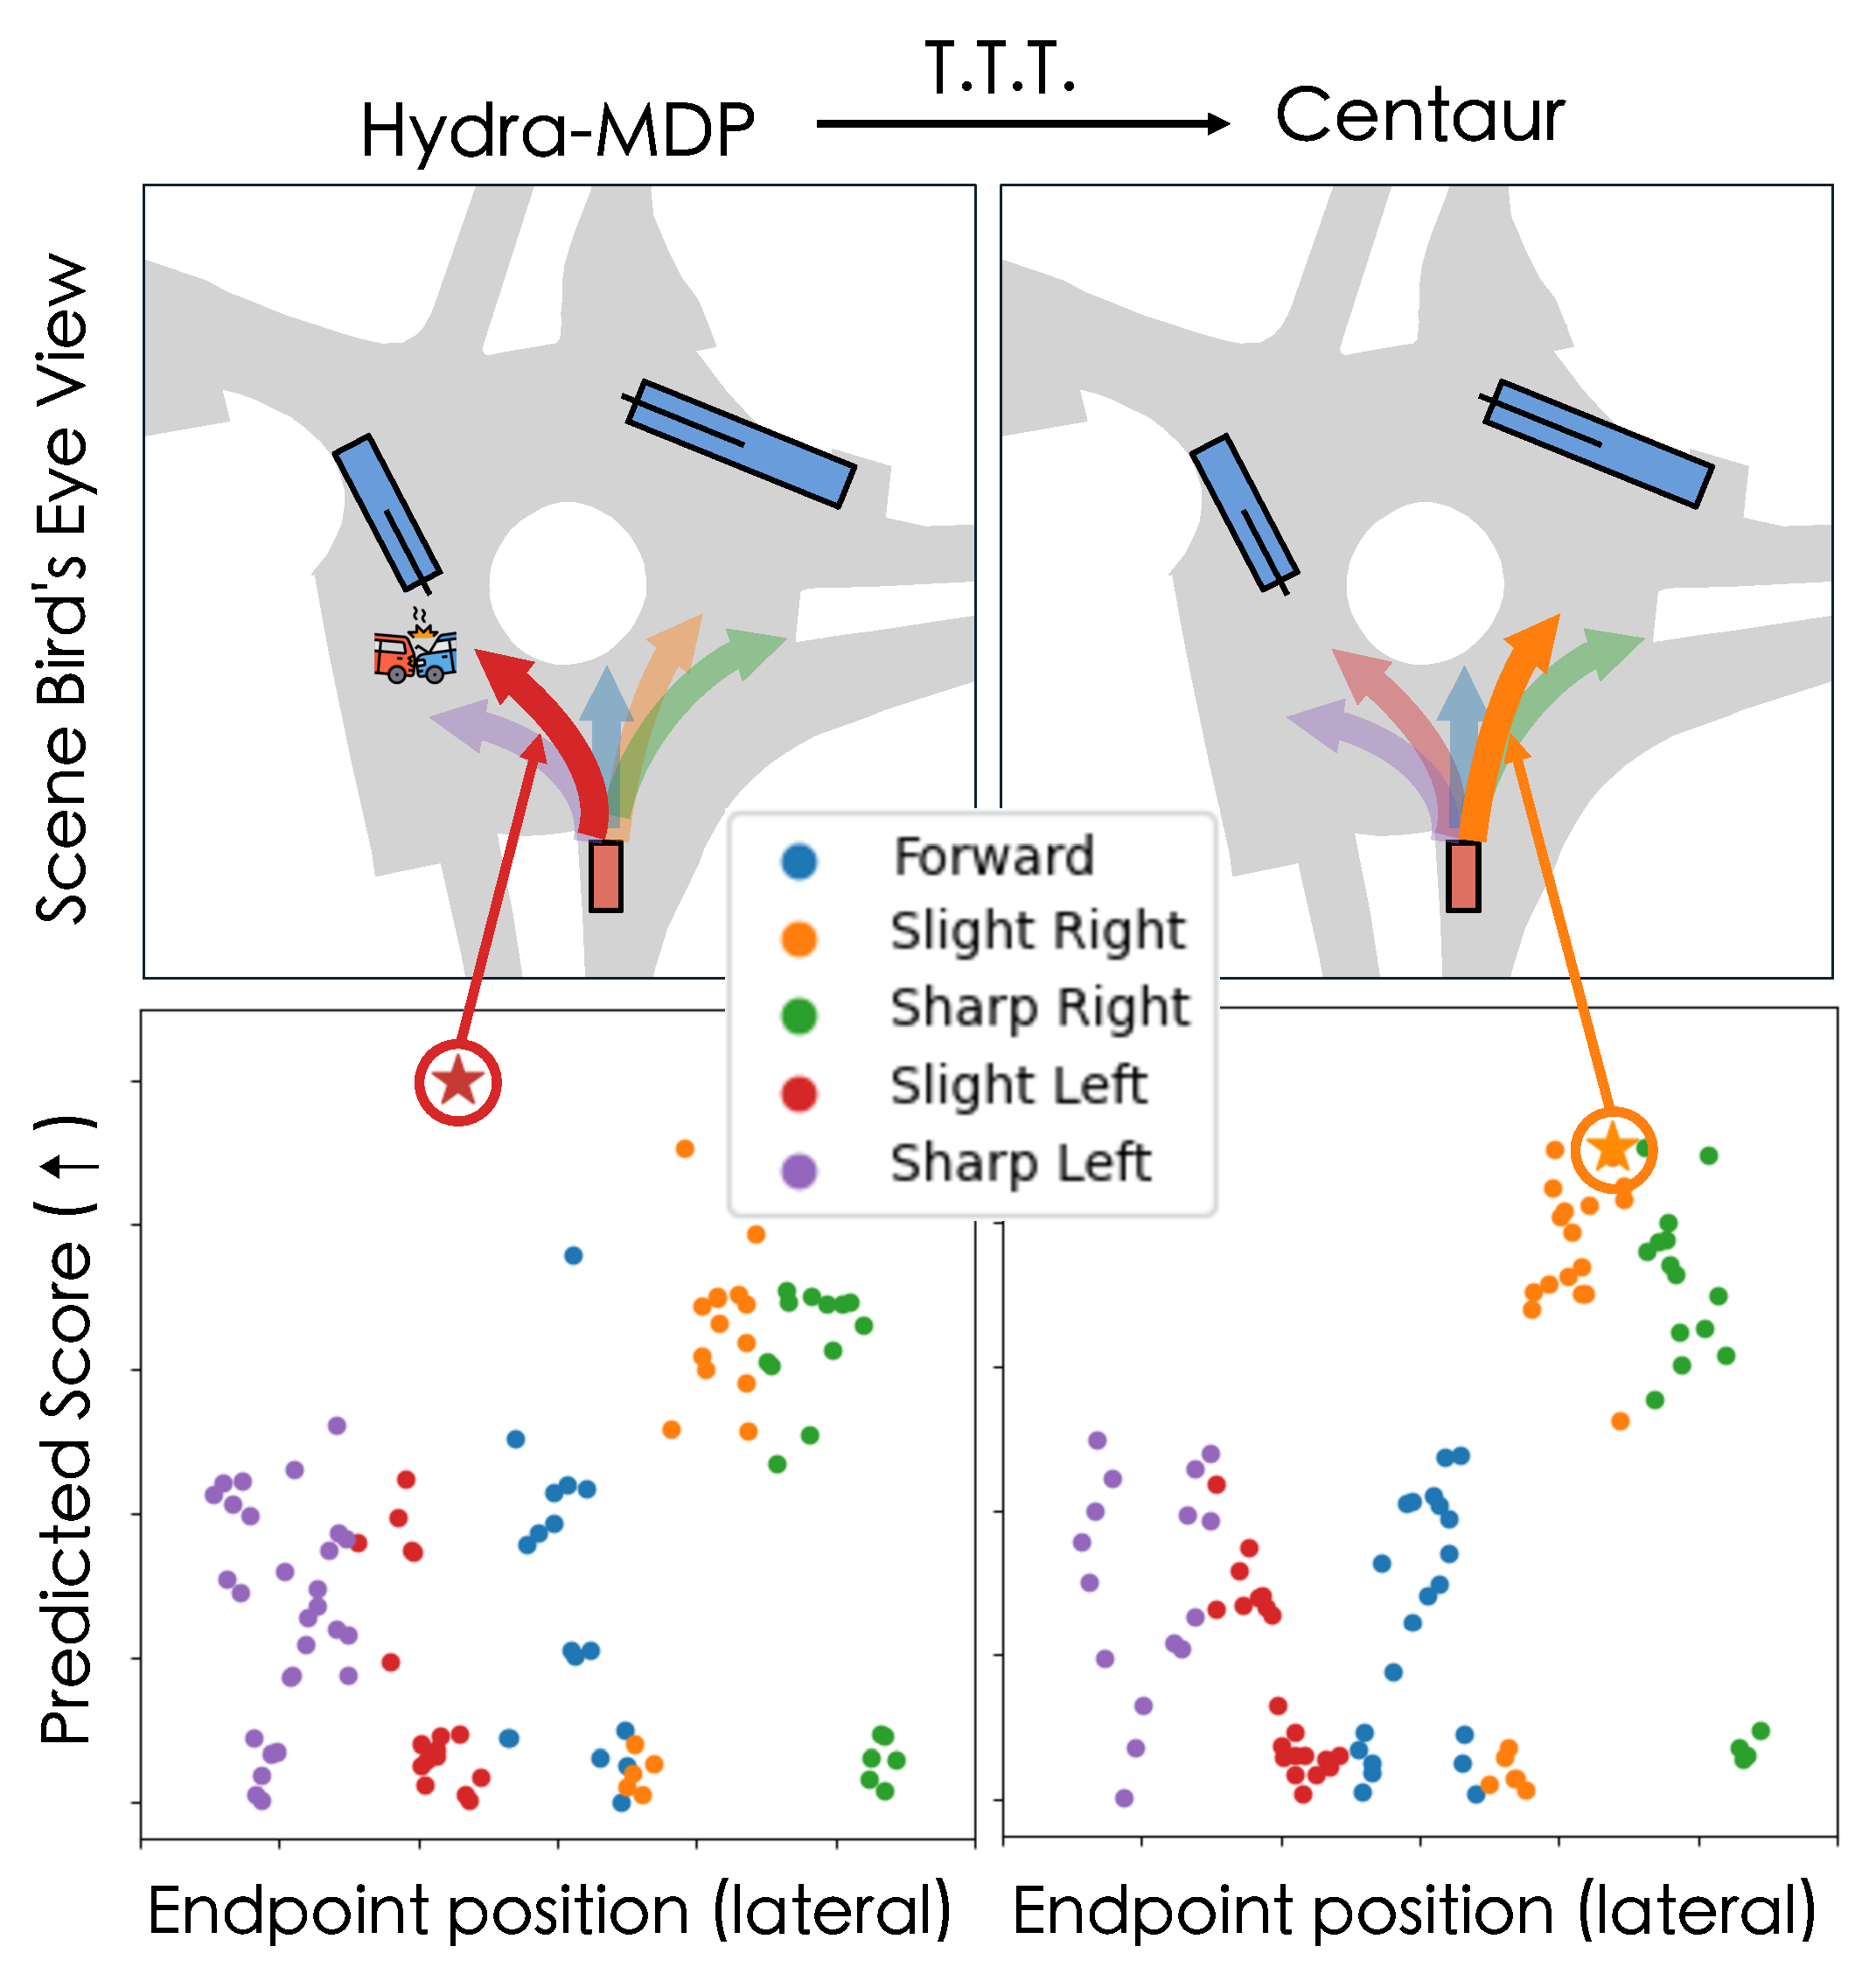
\includegraphics[width=0.55\textwidth]{ch-centaur/images/main_fig_v15.pdf}
  \caption[Reducing entropy when uncertain with test-time training]{\textbf{Reducing entropy when uncertain with test-time training (TTT).} The end-to-end planner Hydra-MDP~\cite{li2024hydramdp}, state-of-the-art on \texttt{navtest}~\cite{dauner2024navsim}, predicts a score for every trajectory in a fixed set. In the scatter plots, trajectory scores are plotted against their lateral endpoint position and clustered into five categories (coloured arrows in the upper visualisations). Hydra-MDP selects the trajectory with the highest predicted score ($\bigstar$) as its output. \textbf{Left:} In this roundabout, it selects a high-scoring outlier in the cluster `slight left', where the average score is low, indicating high uncertainty. \textbf{Right:} This uncertainty is measured by the proposed Cluster Entropy, which Centaur minimises via gradient descent (TTT). The result is a more confident planner (with less entropy) that in this scene prefers `slight right' turns, avoiding a collision.}
  \label{centaur:fig:teaser}
\end{figure}

Safe interaction with other road users and robustness in unforeseen situations are vital as autonomous vehicles increasingly share public streets with human-driven vehicles~\cite{shalevshwartz2017rss,liu2024curse}. End-to-end planners are increasingly studied for their scalability and empirical performance~\cite{chitta2023transfuser,hu2023uniad,weng2024paradrive,li2024hydramdp,chen2024e2esurvey,li2023open}. In practice, they may be combined with fallback actions and feasibility or collision checks~\cite{chitta2023transfuser,vitelli2022safetynet,waywe2024ad2}. Such safeguards require explicit engineering choices and can change the progress--safety trade-off; their effectiveness depends on the design and evaluation protocol.

Another approach refines a planned trajectory at test time with an expert-crafted cost~\cite{hu2023uniad,Hu2023hoplan}. Such objectives can use explicit representations including drivable-area maps and predicted motions to penalise off-road or colliding trajectories. Their labels, modelling assumptions and runtime differ from those of a trajectory-scoring planner. This motivates evaluating a complementary update objective that uses the planner's own predicted scores without requesting new labels or evaluating a new scene-dependent safety cost at test time.

Centaur achieves this through test-time training~\cite{sun2024learning,liang2025ttasurvey}, which computes a gradient of the network weights to minimise an objective defined on a small dataset collected during deployment~\cite{wang2022cotta,liang2025ttasurvey,Gao2024fstta}. In contrast to test-time trajectory optimisation with explicit representations and expert-designed cost functions, the TTT objective of Centaur optimises the network weights to reduce planning uncertainty, which can be estimated in an unsupervised manner. Furthermore, although Centaur trains at test time, it performs gradient computation and inference asynchronously and in parallel, which keeps the overhead in runtime latency minimal.

Defining a planning uncertainty that enables TTT is, however, non-trivial under the historically prevalent paradigm of trajectory regression in end-to-end driving~\cite{hu2023uniad,chitta2023transfuser,weng2024paradrive,li2024ego}, in which the planner directly regresses the desired trajectory from sensor inputs. Existing work on TTT focuses on classification~\cite{Gao2024fstta,wang2021tent}, where the objective is typically the entropy of the prediction, a quantity that is not easy to compute in a regression setting. An emerging class of end-to-end driving methods based on trajectory scoring~\cite{li2024hydramdp,Sadat2020P3,Casas2021mp3} instead assigns numerical scores to multiple trajectory candidates, much like a classifier. Focusing on this class, Centaur introduces Cluster Entropy, which aggregates the candidate trajectory scores of the planner into clusters based on driving direction and computes the entropy of this simple and interpretable distribution.

Fig.~\ref{centaur:fig:teaser} illustrates the approach with Hydra-MDP~\cite{li2024hydramdp}, a trajectory-scoring planner. In the complex scene shown, the vehicle is entering a roundabout. After TTT, the distribution of high-scoring trajectories becomes more concentrated on the safer behaviour of a right turn, which helps the planner avoid illegally turning left into oncoming traffic. Besides its use for TTT, Cluster Entropy can also flag situations in which the model is likely to fail: at a fixed threshold, it gives the highest true-positive rate among the compared uncertainty measures. This suggests its potential as a mechanism for alerting human drivers to intervene, although the evidence is limited (Section~\ref{centaur:sec:failure}).

Finally, as planners draw closer to the logged human-trajectory reference on existing benchmarks, a single aggregate score says little about where they still fail. To advance safe autonomous driving, we therefore construct \texttt{navsafe}, a benchmark of edge cases and challenging driving scenarios, with a semi-automated data curation pipeline that involves human annotation and verification to sample safety-critical scenarios. Evaluating state-of-the-art planners, including Centaur, on \texttt{navsafe} reveals new insights into their strengths and weaknesses, as well as a substantial gap to the logged human-trajectory reference.

%-------------------------------------------------------------------------------
\section{Related Work}\label{centaur:sec:related}

\paragraph{End-to-end autonomous driving.} End-to-end autonomous driving represents a paradigm shift in autonomous vehicle technology~\cite{chen2024e2esurvey}. Its goal is to map raw sensor inputs directly to vehicle control outputs with neural networks, bypassing traditional modular components such as separate perception, planning and control systems~\cite{Prakash2021transfuser,chitta2021neat,jaeger2023hidden,zimmerlin2024tf,chen2024vadv2,jiang2023vad,hu2023uniad,hu2022model,jia2023think,wang2023drivedreamer,jia2023driveadapter,li2024hydramdp,liao2025diffusiondrive}, including the occupancy-based approach of Chapter~\ref{ch:occnet}~\cite{sima2023occnet}.

\paragraph{End-to-end planner deployment.} Obtaining trustworthy outputs from an end-to-end system during deployment is challenging. Rule-based planners and fallback layers are common ways to guard planning outputs. UniAD~\cite{hu2023uniad} refines a plan with an explicit cost, TransFuser~\cite{chitta2023transfuser} applies forced braking when LiDAR detects obstacles, and SafetyNet~\cite{vitelli2022safetynet} checks dynamic feasibility, legality and collisions before selecting from scene-conditioned fallback trajectories. The baseline implemented in this chapter is narrower: an uncertainty-triggered replacement from a fixed bank of twenty globally selected trajectories (Section~\ref{centaur:sec:setup}). It is inspired by fallback safeguards but is not a full reimplementation of SafetyNet. Conclusions from this baseline are therefore limited to the measured protocol.

\paragraph{Test-time compute and training.} Leveraging test-time compute has recently emerged as an important way to strengthen reasoning capabilities~\cite{openaio1}. In addition, test-time adaptation and training techniques~\cite{liang2025ttasurvey} have shown considerable potential in computer vision~\cite{sun2024learning,hakim2023clust3,marsden2024universal}, multimodal learning~\cite{shu2022test,yoon2024c}, vision-language navigation~\cite{Gao2024fstta}, trajectory prediction~\cite{park2024t4p}, robot manipulation~\cite{hansen2021pad} and long-context large language models~\cite{sun2024learning}. The key idea of these approaches is to minimise entropy or related proxies at test time. Centaur is aligned in spirit with them and was, to the best of our knowledge, at the time of publication, the first work to explore the potential of test-time training via uncertainty measurement for the vehicle motion planning task.

Further related work on Hydra-MDP and ensembling, semantic entropy, safety-critical scenario benchmarks and evidential uncertainty is discussed in Appendix~\ref{centaur:app:related}.

%-------------------------------------------------------------------------------
\section{Method}\label{centaur:sec:method}

This section presents the pipeline of Centaur, which focuses on deploying a planner that has already been trained, as shown in Fig.~\ref{centaur:fig:pipeline}. Section~\ref{centaur:sec:prelim} introduces the planning formulation, Section~\ref{centaur:sec:ce} defines Cluster Entropy, and Section~\ref{centaur:sec:ttt} describes how Cluster Entropy is minimised at test time.

\begin{figure}[t]
  \centering
  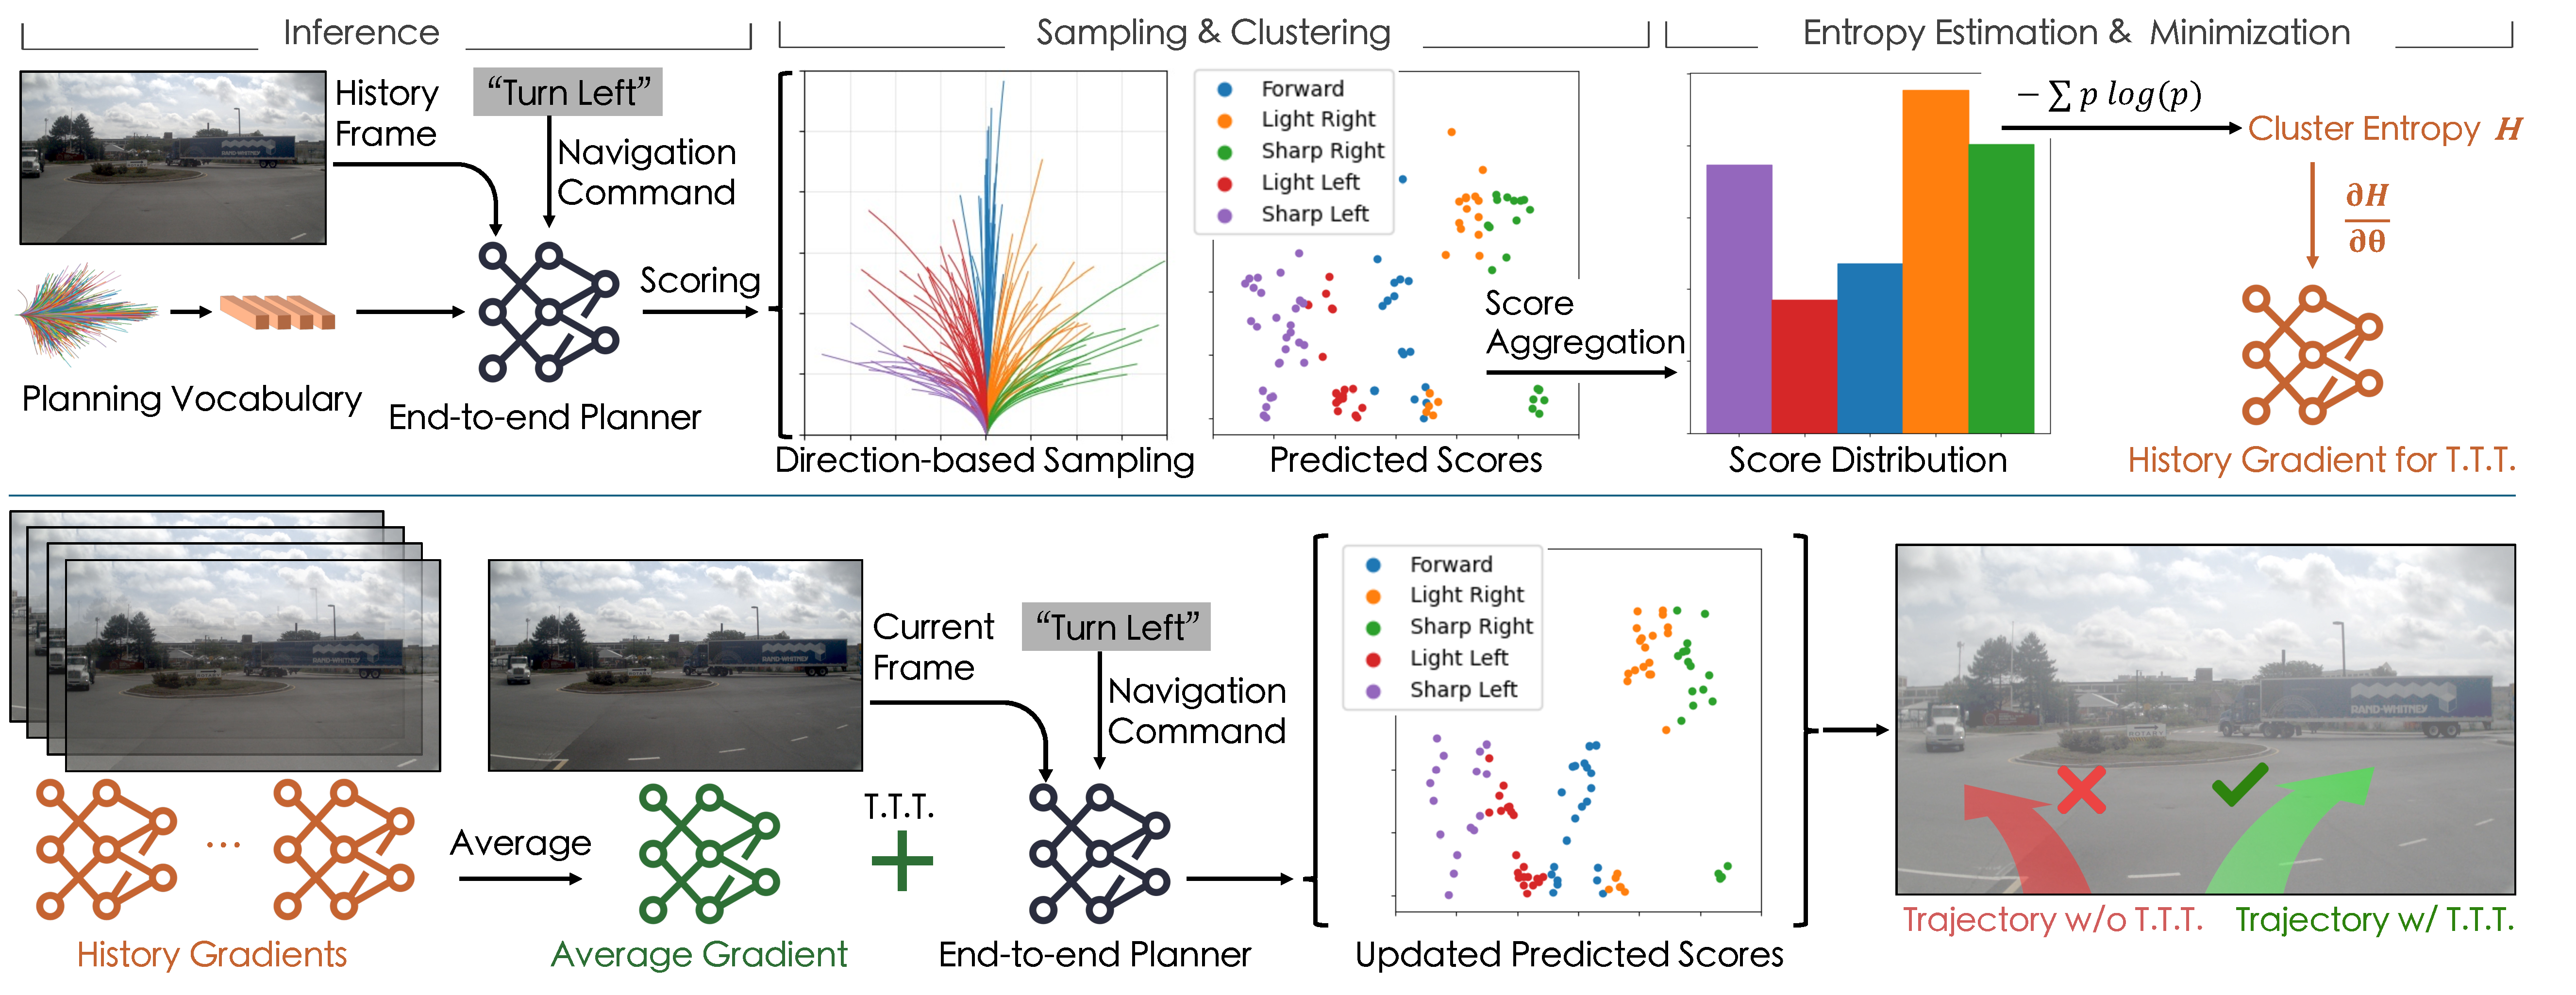
\includegraphics[width=\textwidth]{ch-centaur/images/pipeline_v11.pdf}
  \caption[Test-time training in Centaur]{\textbf{Test-time training (TTT) in Centaur.} \textbf{Top:} A trained end-to-end planner scores trajectories from the planning vocabulary for frames observed during testing. A subset of these trajectories is sampled and clustered based on driving direction. After the predicted scores are aggregated over clusters, a Cluster Entropy is calculated to reflect the uncertainty, and a gradient for Cluster Entropy minimisation is obtained via backpropagation. \textbf{Bottom:} Gradients from historical frames are accumulated and used to update the planner, improving its performance.}
  \label{centaur:fig:pipeline}
\end{figure}

\subsection{Preliminaries}\label{centaur:sec:prelim}

End-to-end self-driving methods seek a policy $\pi$ that outputs decisions such as desired trajectories $\mathbf{t}$ from sensor inputs $\mathbf{x}$ and a navigation command $\mathbf{c}$. A trajectory $\tilde{\mathbf{t}}=(\mathbf{p}_0,\ldots,\mathbf{p}_N)$ is a sequence of future bird's-eye-view positions. \emph{Trajectory regression} predicts it directly from demonstrations. Centaur instead focuses on \emph{trajectory scoring}, where a planner ranks a fixed vocabulary; examples include Hydra-MDP~\cite{li2024hydramdp}, VADv2~\cite{chen2024vadv2} and RAD~\cite{gao2025rad}. Appendix~\ref{centaur:app:regression} describes the source adaptation to regression planners.

\paragraph{Trajectory scoring.} In this formulation, the planner outputs a set of scalar \emph{score features} $\{s_j\}_{j=1}^k$ for a \emph{planning vocabulary} of $k$ different trajectories. The score features numerically capture different aspects of desired driving behaviour, such as avoiding collisions and making progress. They can be aggregated into a single final score via an aggregation function $\phi$. During inference, the trajectory with the largest predicted final score is selected:
\begin{equation}
  \label{centaur:eq:multi-score-output}
  \{s_j\}_{j=1}^k = \{ \pi_\theta(\mathbf{t}_j, \mathbf{x}_0, \mathbf{c}_0) \}_{j=1}^k,
\end{equation}
\begin{equation}
  \label{centaur:eq:cost-select}
  \hat{\mathbf{t}}_0 = \argmax_{\mathbf{t}_j} \{\phi(s_j)\}_{j=1}^k.
\end{equation}
As a result of this design, the planner is inherently multi-modal, and the distribution of scores over the planning vocabulary provides a way to represent planning uncertainty. For this type of planner, learning the policy parameters $\theta$ can be formulated as
\begin{equation}
  \label{centaur:eq:objective-score}
  \argmin_{\theta} \mathbb{E}_{(\mathbf{t},\mathbf{x},\mathbf{c})\sim D_{kd}} \left[\mathcal{L}_{kd}\big(e(\mathbf{t},\mathbf{x},\mathbf{c}), \pi_\theta(\mathbf{t},\mathbf{x},\mathbf{c})\big)\right],
\end{equation}
where $e$ is an expert algorithm that can provide ground-truth score features for any sampled trajectory, and $D_{kd} = \{(\mathbf{t}, \mathbf{x}, \mathbf{c}), \dots\}$ is a knowledge distillation dataset generated by sampling this expert algorithm for different inputs, typically in a driving simulator~\cite{caesar2021nuplan,dosovitskiy2017carla} or a world model~\cite{yang2024genad,gao2024vista}. In practice, the score features are normalised to the range $(0,1)$, and $\mathcal{L}_{kd}$ is implemented as a cross-entropy loss. The complete training loss of the Hydra-MDP implementation used in this chapter, which adds an imitation term, is given in Appendix~\ref{centaur:app:scoring}.

\subsection{Cluster Entropy}\label{centaur:sec:ce}

In essence, the scoring procedure of Eqs.~\eqref{centaur:eq:multi-score-output} and~\eqref{centaur:eq:cost-select} acts as a classifier over the $k$ classes of the planning vocabulary. We formulate a new uncertainty measure, Cluster Entropy, to translate this intuition into an unsupervised training objective for end-to-end planning, which, unlike Eq.~\eqref{centaur:eq:objective-score}, does not require an expert algorithm. The key challenge is that the planning vocabulary is often very large, typically encompassing several thousand possible trajectories. Even in simple driving scenarios, many neighbouring trajectories in the vocabulary therefore receive nearly identical scores. Simply minimising the entropy of the distribution of scores over the vocabulary would yield an objective that encourages the model to avoid trajectories with a larger number of nearby neighbours in the vocabulary, \eg driving straight. Such a naive entropy is therefore unsuitable for uncertainty estimation in this setting. Cluster Entropy instead proceeds in three steps.

\paragraph{Trajectory candidates.} First, we sample a set of $M$ trajectory candidates $\{\mathbf{t}_m\}_{m=1}^M$ from the planning vocabulary, where $M \ll k$. The sampling is weighted to prioritise candidates that have a high average score according to the expert algorithm $e$; the sampling weights are specified in Appendix~\ref{centaur:app:entropy}. The resulting objective is therefore conditional on an expert-scored candidate bank rather than entirely free of privileged training information. Full Entropy applies directly to the selected candidates; the next two steps form a coarser direction-level measure.

\paragraph{Direction-based sampling.} Next, we use domain-specific criteria to select trajectory anchors from the $M$ candidates. Following DriveLM~\cite{sima2024drivelm}, we select five anchors: \texttt{sharp left}, \texttt{slight left}, \texttt{forward}, \texttt{slight right} and \texttt{sharp right}. The \texttt{sharp left} and \texttt{sharp right} anchors, the candidates with the largest lateral offsets, are selected first. The \texttt{slight left} and \texttt{slight right} anchors are the candidates whose lateral offsets are closest to half of those of \texttt{sharp left} and \texttt{sharp right}, and \texttt{forward} is the candidate with the smallest lateral offset.

\paragraph{Score aggregation.} Let $q_j=\phi(s_j)$ be the scalar final score used by the planner to rank candidate $j$. The source description sums these final scores within each direction cluster, so we write $\mathit{score}_a=\sum_{j:\,\mathbf{t}_j\in\mathcal{C}_a}q_j$. The $q_j$ values must be nonnegative with a positive total for normalisation to define a categorical distribution; the implementation reports normalised score features in $(0,1)$, but the exact scalarisation should be checked with the released code. Cluster Entropy is then
\begin{equation}
  \label{centaur:eq:ce}
  p_a = \frac{\mathit{score}_a}{\sum_{a'=1}^{5} \mathit{score}_{a'}}, \qquad
  H(\mathbf{x}) = -\sum_{a=1}^{5} p_a \log p_a .
\end{equation}
Since the distribution has five outcomes, $H$ ranges from $0$ to $\ln 5$. This is a \emph{cluster score-mass entropy}: if candidate scores are equal, $p_a=|\mathcal{C}_a|/M$, so unequal cluster sizes affect it. Direction clustering reduces the dimensionality of the vocabulary but does not make the objective invariant to candidate density. The experiments do not isolate this effect with equal-cardinality or cluster-mean alternatives.

\subsection{Test-Time Training}\label{centaur:sec:ttt}

Equipped with this unsupervised training objective, our goal is to minimise uncertainty at test time, which is the key idea of TTT approaches in the literature. We follow the standard practice of performing a single step of gradient descent to update the network parameters $\theta$~\cite{Gao2024fstta}, using the Cluster Entropy $H(\mathbf{x})$ as the objective function. Specifically, given $H(\mathbf{x})$ calculated after a forward pass through $\pi_\theta$, we obtain the gradient $\frac{\partial H}{\partial \theta}$ by backpropagation. Instead of directly updating $\theta$ with this gradient, however, we store $\frac{\partial H}{\partial \theta}$ in a buffer of length $F=4$, as shown in Fig.~\ref{centaur:fig:pipeline} (bottom). At time step $i$, we update the network using the average $\{\frac{\partial H}{\partial \theta}\}_{avg}$ of all gradients currently in the buffer, obtaining
\begin{equation}
  \label{centaur:eq:ttt}
  \hat{\theta}_i = \theta - \eta \left\{\frac{\partial H}{\partial \theta}\right\}_{avg},
\end{equation}
where $\eta$ is the learning rate. The source description states that historical gradients are averaged and applied before inference on the next frame. It does not specify whether those gradients are evaluated at the base or previously adapted parameters, or when parameters and buffers reset. The high-level procedure is therefore reported here without presenting the earlier pseudocode as a complete reproducible implementation.

\paragraph{Deployment.} The source description applies only gradients from earlier frames before the current inference, allowing gradient calculation and inference to be scheduled on separate hardware. Because the exact parameter/reset semantics are unavailable, this thesis does not claim that Algorithm~\ref{centaur:eq:ttt} is sufficient to reproduce the implementation. The measured end-to-end latency, including gradient calculation, is reported in Section~\ref{centaur:sec:latency}.

%-------------------------------------------------------------------------------
\section{\texorpdfstring{\texttt{navsafe}}{navsafe}: A Safety-Critical Scenario Set}\label{centaur:sec:navsafe}

\begin{figure}[t]
  \centering
  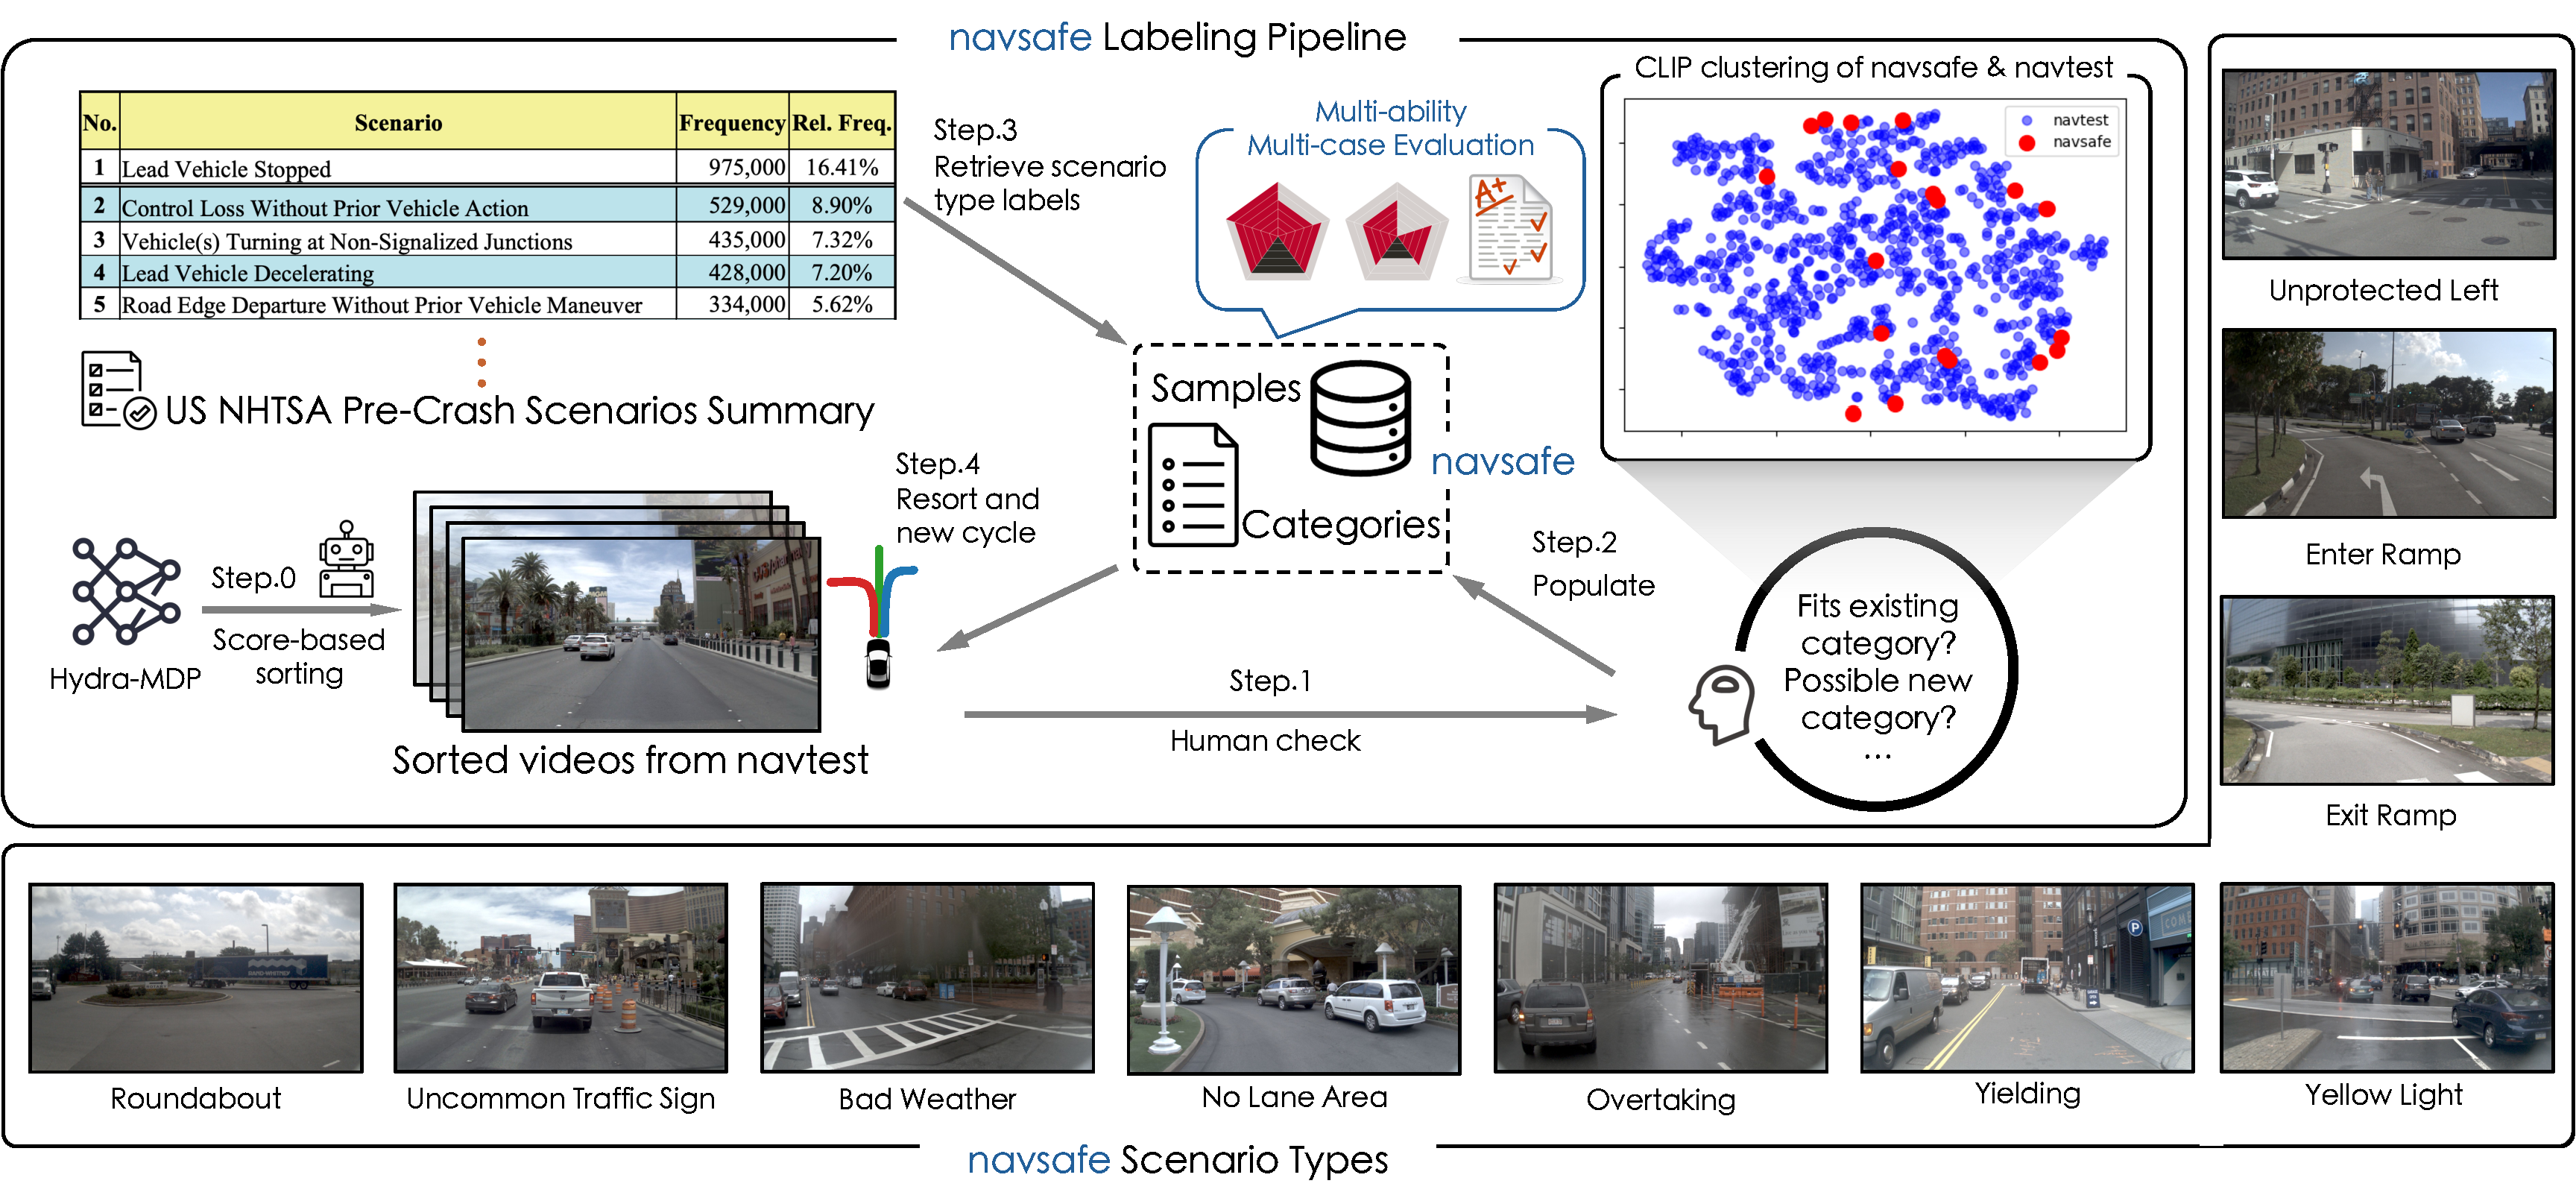
\includegraphics[width=\textwidth]{ch-centaur/images/navsafe_v12.pdf}
  \caption[The \texttt{navsafe} benchmark]{\textbf{\texttt{navsafe}.} Definitions of safety-critical cases from NHTSA (National Highway Traffic Safety Administration) material~\cite{najm2007pre} are used to search \texttt{navtest} for matching frames. Following human checks, these frames form \texttt{navsafe}. CLIP-based clustering~\cite{ilharco2021openclip} of \texttt{navsafe} alongside \texttt{navtest} shows that \texttt{navsafe} consists of frames from the peripheral regions of the distribution.}
  \label{centaur:fig:navsafe}
\end{figure}

The split is a targeted diagnostic rather than a prevalence sample. Its search begins by sorting \texttt{navtest} clips by Hydra-MDP performance and then adding human-verified examples to NHTSA-inspired categories. This makes it useful for inspecting difficult frames, but it also enriches for Hydra-MDP failures and can bias comparisons involving methods derived from Hydra-MDP. It should not be used to estimate performance on naturally occurring safety events.

\paragraph{NAVSIM.} The framework on which \texttt{navsafe} is built is primarily designed to capture scenarios with significant changes in driving behaviour, where the historical trajectory of the ego vehicle does not allow for an accurate extrapolation of the future plan. It is split into two parts, \texttt{navtrain} and \texttt{navtest}, which contain 1,192 logs (103,288 frames) and 136 logs (12,146 frames), respectively. In NAVSIM, driving agents are required to plan a trajectory as a sequence of future positions spanning a horizon of 4 seconds. The input to an agent includes 1.5 seconds of past history (resulting in 4 frames of data) from onboard camera and LiDAR sensors, as well as the vehicle's current speed, acceleration and navigation command, collectively referred to as the ego status. We retain these default NAVSIM settings for evaluation on \texttt{navsafe}.

\paragraph{Construction criteria.} Fig.~\ref{centaur:fig:navsafe} illustrates the data curation process for \texttt{navsafe}. The US NHTSA holds a collection of traffic accidents reported every year across the nation, which is shared publicly via a pre-crash scenario typology for crash avoidance research~\cite{najm2007pre}. It includes a wide variety of pre-crash scenario types, ranging from common ones such as ``Lead Vehicle Stopped'' to uncommon ones such as ``Animal Crash With Prior Vehicle Maneuver''. Supported by summary statistics on the types of pre-crash scenarios~\cite{thorn2018framework,najm2007pre}, \texttt{navsafe} is curated to highlight the safety-critical scenarios in which modern end-to-end planners could fail. We construct it with the following steps:
\begin{enumerate}[label={Step~\arabic*.}, start=0, leftmargin=*]
  \item Sort the video clips in the \texttt{navtest} split by the average performance of a state-of-the-art planner~\cite{li2024hydramdp}.
  \item Check the video clips with human annotators and try to assign frames to new or existing categories in \texttt{navsafe}.
  \item Populate the scenario types with new examples.
  \item Retrieve scenario type labels from the NHTSA file to define scenario types not yet in \texttt{navsafe}.
  \item Re-sort \texttt{navtest} and start a new cycle of the workflow.
\end{enumerate}

\paragraph{Highlights of \texttt{navsafe}.} The benchmark contains 229 of the 12,146 \texttt{navtest} frames in ten categories: ``Roundabout'', ``Yellow light, rush or wait?'', ``Exit ramp'', ``Unprotected left'', ``Enter ramp'', ``Uncommon traffic sign'', ``Overtaking with lane change'', ``No lane area (\eg parking lot)'', ``Bad weather'' and ``Yielding (\eg to pedestrians)''. Per-category scores permit a finer diagnostic than one aggregate. CLIP projections in Fig.~\ref{centaur:fig:navsafe} place many selected frames near peripheral regions of the displayed \texttt{navtest} embedding, but that visualisation is not a density estimate. The experiments compare logged human trajectories and end-to-end planners on this deliberately selected stress set.

%-------------------------------------------------------------------------------
\section{Experiments}\label{centaur:sec:exp}

This section evaluates Centaur on the NAVSIM framework~\cite{dauner2024navsim}, including the official \texttt{navtest} leaderboard and the \texttt{navsafe} scenarios of Section~\ref{centaur:sec:navsafe}.

\subsection{Experimental Setup}\label{centaur:sec:setup}

\paragraph{Metrics.} The experiments adopt NAVSIM's PDM score (PDMS). For each valid frame, NAVSIM v1 simulates the planned trajectory for four seconds, while other road users do not react, and aggregates normalised sub-scores. NAVSIM then averages the per-frame PDMS and each displayed component separately across valid frames:
\begin{equation}
  \label{centaur:eq:pdms}
  \mathrm{PDMS} = \mathrm{NC} \times \mathrm{DAC} \times \left( \frac{5\,\mathrm{TTC} + 2\,\mathrm{C} + 5\,\mathrm{EP}}{12} \right),
\end{equation}
where NC (No at-fault Collision) and DAC (Drivable Area Compliance) are multiplicative penalties, and EP (Ego Progress), C (Comfort) and TTC (Time-to-Collision) form a weighted average. The quantities lie in $[0,1]$ in the evaluator and are displayed as percentages. The public v1.0 devkit additionally includes Driving Direction Compliance as a multiplicative penalty, whereas v1.1 removes it from the default score; the exact devkit commit and resolved configuration used for each local table therefore need to be pinned. TTC identifies whether a constant-velocity projection would collide within one second at any point on the planned trajectory.

\paragraph{Base model.} Designed specifically for NAVSIM, our base model Hydra-MDP~\cite{li2024hydramdp} takes LiDAR points as input, which are splatted onto the BEV plane and encoded by a ResNet34~\cite{he2016deep}. These features are fused with image features extracted by a \mbox{V2-99}~\cite{park2021pseudo} backbone via the sensor fusion modules of TransFuser~\cite{chitta2023transfuser}. The decoder then predicts scores for a planning vocabulary of $k=8192$ trajectories. The score functions output by the decoder are the five sub-scores (NC, DAC, EP, C and TTC) considered in the NAVSIM evaluation. Additional experiments with the more lightweight TransFuser~\cite{chitta2023transfuser}, which performs trajectory regression instead of scoring, are provided in Appendix~\ref{centaur:app:ablations} and summarised in Section~\ref{centaur:sec:ablations}.

\paragraph{Deployment strategy.} As a deliberately simple fallback baseline, we implement uncertainty-triggered replacement from a fixed trajectory bank, inspired by the fallback idea in SafetyNet~\cite{vitelli2022safetynet}. This is not SafetyNet's scene-conditioned feasibility and collision-checking pipeline. We calculate the average PDMS of each trajectory in Hydra-MDP's planning vocabulary and retain the top 20. At inference, an uncertainty value above a threshold triggers replacement by the bank trajectory closest to the prediction in $L_2$ distance. The thresholds are reported with Table~\ref{centaur:tab:fail_class}; the exact relationship between its detection events and the aggregate fallback columns is part of the record check below.

\paragraph{Uncertainty measures.} We compare Cluster Entropy with three baselines. For \textbf{KL Divergence}, we obtain the predicted categorical distribution over the planning vocabulary ($k=8192$ classes) for each score function (NC, DAC, EP, C and TTC), then calculate the KL divergence between each pair of distributions and sum over all pairs. \textbf{Full Entropy}~\cite{shannon1948entropy} is calculated like Cluster Entropy, but skips the clustering of the $M=100$ candidates into five clusters and simply computes the entropy of the full 100-way candidate score distribution. \textbf{Semantic Entropy} is our adaptation of semantic uncertainty~\cite{kuhn2023semantic} to autonomous driving. Its calculation is again similar to that of Cluster Entropy, but the candidates are clustered in a feature space in which each trajectory is represented by its predicted scores $s_j$ (details in Appendix~\ref{centaur:app:entropy}). For compactness, TTT for Hydra-MDP with Semantic Entropy, the baseline used most frequently in the experiments, is referred to as \textbf{Hydra-SE}.

\paragraph{Implementation.} Except for Table~\ref{centaur:tab:navtest_all}, the source reports NAVSIM v1.0 for training and local evaluation; the official leaderboard in Table~\ref{centaur:tab:navtest_all} uses v1.1. The local comparisons are single runs, while the leaderboard entries are means over three seeds. The exact local devkit commit, resolved scoring configuration, valid-token manifest and output schema are unavailable, as are the buffer reset boundary and gradient evaluation point; these omissions limit exact reproduction. Hydra-MDP~\cite{li2024hydramdp} is trained on \texttt{navtrain} for 20 epochs on 8 NVIDIA A100 GPUs with a total batch size of 256. AdamW uses learning rate $10^{-4}$ and no weight decay. The source reports $M=100$ candidates, one gradient step with $\eta=10^{-4}$ and $F=4$ history frames, updating the score decoder while freezing the perception backbones.

\subsection{Impact of Test-Time Training on \texorpdfstring{\texttt{navtest}}{navtest}}\label{centaur:sec:results}

\begin{table}[t]
  \centering
  \caption[Impact of test-time training on \texttt{navtest}]{\textbf{Impact of TTT on \texttt{navtest}.} Source-reported single-run NAVSIM v1.0 values are preserved. The four fixed-bank fallback rows require the aggregation check below before supporting a comparison with TTT. Three-seed v1.1 results are given in Table~\ref{centaur:tab:navtest_all}.}
  \label{centaur:tab:navtest_ablation}
  \begin{adjustbox}{max width=\textwidth}
  \begin{tabular}{l|ll|rrrr|rr}
    \toprule
    \textbf{Model} & \textbf{Deployment} & \textbf{Uncertainty} & \textbf{NC} $\uparrow$ & \textbf{DAC} $\uparrow$ & \textbf{EP} $\uparrow$ & \textbf{C} $\uparrow$ & \textbf{TTC} $\uparrow$ & \textbf{PDMS} $\uparrow$ \\
    \midrule
    \multirow{7}{*}{Hydra-MDP~\cite{li2024hydramdp}} & - & - & $98.4$ & $97.8$ & $\mathbf{86.5}$ & $100.0$ & $93.9$ & $90.3$ \\
    \cmidrule(lr){2-9}
    & \multirow{4}{*}{Fixed-bank fallback} & KL Divergence & $99.1$ & $99.2$ & $9.6$ & $100.0$ & $96.7$ & $63.1$ \\
    & & Full Entropy & $99.6$ & $99.4$ & $13.2$ & $100.0$ & $99.1$ & $65.9$ \\
    & & Semantic Entropy & $\mathbf{99.7}$ & $\mathbf{99.5}$ & $10.4$ & $100.0$ & $98.9$ & $65.3$ \\
    & & Cluster Entropy & $\mathbf{99.7}$ & $\mathbf{99.5}$ & $8.2$ & $100.0$ & $\mathbf{99.3}$ & $64.2$ \\
    \cmidrule(lr){2-9}
    & \multirow{2}{*}{TTT} & KL Divergence & $98.9$ & $98.1$ & $86.0$ & $100.0$ & $94.4$ & $91.5$ \\
    & & Full Entropy & $99.3$ & $98.5$ & $85.7$ & $100.0$ & $97.1$ & $91.8$ \\
    \midrule
    Hydra-SE & TTT & Semantic Entropy & $99.2$ & $98.5$ & $85.7$ & $100.0$ & $97.1$ & $91.8$ \\
    \textbf{Centaur (Ours)} & TTT & Cluster Entropy & $99.5$ & $98.9$ & $85.9$ & $100.0$ & $98.0$ & $\mathbf{92.6}$ \\
    \midrule
    \textit{Human Trajectory} & - & - & $\mathit{100.0}$ & $\mathit{100.0}$ & $\mathit{87.5}$ & $\mathit{99.9}$ & $\mathit{100.0}$ & $\mathit{94.8}$ \\
    \bottomrule
  \end{tabular}
  \end{adjustbox}
\end{table}

Table~\ref{centaur:tab:navtest_ablation} shows the main results, examining two key aspects: the deployment strategy and the uncertainty measure.

\paragraph{Status of the fixed-bank fallback rows.} Under the public NAVSIM v1 scorer, each valid frame satisfies
$\mathrm{PDMS}\leq(5\,\mathrm{TTC}+2\,\mathrm{C}+5\,\mathrm{EP})/12$, and the evaluator then takes an equal-weight mean of each column. The displayed fallback rows exceed the corresponding bounds from their displayed EP, C and TTC means by 2.1--3.1 points. Rounding cannot explain this gap. The original per-token component scores, valid and trigger flags, and exact scorer configuration are unavailable, so the discrepant quantity cannot be identified. The values are retained as source records but are not used to establish that TTT is generally preferable to fallback safeguards.

\paragraph{Deployment strategy.} The TTT rows preserve high EP while improving the reported safety-related sub-scores. By contrast, the source-reported fixed-bank fallback rows show higher NC, DAC and TTC but much lower EP. Because their column aggregation is unresolved, the magnitude of that trade-off is not interpreted here. This restricted baseline also cannot represent the full set of contextual checks and generated trajectories used by SafetyNet. The comparison supports TTT on the reported NAVSIM protocol, not a claim that learned adaptation supersedes safety filters in general.

\paragraph{Uncertainty measure.} In this single-run comparison, Centaur improves by 2.3 PDMS over Hydra-MDP and by 0.8 PDMS over Hydra-SE (92.6 \vs 91.8). The margin over Hydra-SE shrinks to 0.23 PDMS in the three-seed NAVSIM v1.1 results (Section~\ref{centaur:sec:leaderboard}), less than Centaur's reported standard deviation. All four tested uncertainty objectives improve over the single-run Hydra-MDP score, so the evidence more strongly supports entropy-style TTT in this setting than a distinct accuracy advantage of Cluster Entropy. The direction clusters provide a coarse view of how predicted score mass is distributed across steering modes. They should not be read as faithful explanations of the downstream decision.

\subsection{Failure Identification}\label{centaur:sec:failure}

\begin{table}[t]
  \centering
  \caption[Failure identification on \texttt{navtest}]{\textbf{Failure identification.} A frame is positive when a source-defined safety sub-score failure occurs; the exact predicate remains to be recovered. Uncertainty above a fixed threshold flags a likely failure. Cluster Entropy has the highest reported TPR among the compared measures, but every method has lower accuracy than Select None. AUROC and AUPRC were not reported.}
  \label{centaur:tab:fail_class}
  \begin{tabular}{l|c|rr}
    \toprule
    \textbf{Uncertainty} & \textbf{Threshold} & \textbf{TPR} $\uparrow$ & \textbf{Acc.} $\uparrow$ \\
    \midrule
    KL Divergence & $1500$ & $41.3$ & $68.3$ \\
    Full Entropy & $0.8$ & $61.7$ & $70.4$ \\
    Semantic Entropy & $0.8$ & $62.5$ & $72.2$ \\
    \textbf{Cluster Entropy (Ours)} & $0.8$ & $\mathbf{62.8}$ & $\mathbf{73.6}$ \\
    \midrule
    \textit{Select All} & - & $\mathit{100.0}$ & $\mathit{15.6}$ \\
    \textit{Select None} & - & $\mathit{0.0}$ & $\mathit{84.4}$ \\
    \bottomrule
  \end{tabular}
\end{table}

In this experiment, uncertainty estimates classify source-defined safety failures. The author has clarified that the positive label is a safety sub-score failure rather than necessarily total PDMS zero, but the original Boolean predicate and code are unavailable. The table therefore preserves the source labels without claiming an independently reproduced definition. At $0.8=0.5\ln5$, Cluster Entropy has the highest reported TPR (62.8\%) and accuracy (73.6\%) among the uncertainty measures. The positive prevalence is 15.6\%, so every method remains below the 84.4\% accuracy of Select None; accuracy is uninformative at this imbalance. Because AUROC, AUPRC and confidence intervals were not reported, the result supports only a comparison at the selected operating points.

The reported TTT PDMS orders the uncertainty objectives in the same way as the fixed-threshold TPR/accuracy comparison, with Cluster Entropy highest in both. The fixed-bank fallback columns are not interpreted until the source aggregation and trigger records requested above are recovered. Threshold sweeps for other planners and measures are retained in Appendix~\ref{centaur:app:ablations}.

\subsection{\texorpdfstring{\texttt{navtest}}{navtest} Leaderboard}\label{centaur:sec:leaderboard}

\begin{table}[t]
  \centering
  \caption[The \texttt{navtest} leaderboard]{\textbf{\texttt{navtest} leaderboard.} Official NAVSIM v1.1 \texttt{navtest} leaderboard at the time of the paper's submission (March 2025). We report the mean and standard deviation over 3 independent training runs, as recommended in the leaderboard rules. *The Hydra-MDP entry, which won the 2024 NAVSIM challenge, is a single evaluation of a 3-model ensemble, unlike all other rows.}
  \label{centaur:tab:navtest_all}
  \begin{adjustbox}{max width=\textwidth}
  \begin{tabular}{l|llll|ll}
    \toprule
    \textbf{Model} & \textbf{NC} $\uparrow$ & \textbf{DAC} $\uparrow$ & \textbf{EP} $\uparrow$ & \textbf{C} $\uparrow$ & \textbf{TTC} $\uparrow$ & \textbf{PDMS} $\uparrow$ \\
    \midrule
    \textbf{Centaur (Ours)} & $99.23\pm0.35$ & $\mathbf{98.72\pm0.22}$ & $\mathbf{85.96\pm0.77}$ & $99.97\pm0.03$ & $97.17\pm1.06$ & $\mathbf{92.10\pm0.33}$ \\
    Hydra-SE & $\mathbf{99.32\pm0.05}$ & $98.58\pm0.12$ & $85.42\pm0.07$ & $99.96\pm0.01$ & $\mathbf{97.30\pm0.23}$ & $91.87\pm0.19$ \\
    \midrule
    Hydra-MDP*~\cite{li2024hydramdp} & $99.07$ & $98.29$ & $85.20$ & $\mathbf{100.0}$ & $96.56$ & $91.26$ \\
    TransFuser~\cite{chitta2023transfuser} & $97.78\pm0.10$ & $92.63\pm0.48$ & $78.88\pm0.25$ & $99.98\pm0.01$ & $92.89\pm0.21$ & $83.88\pm0.45$ \\
    LTF~\cite{chitta2023transfuser} & $97.68\pm0.11$ & $92.29\pm0.45$ & $78.33\pm0.53$ & $99.99\pm0.01$ & $93.10\pm0.19$ & $83.52\pm0.55$ \\
    Ego Status MLP~\cite{dauner2024navsim} & $93.09\pm0.12$ & $78.26\pm0.98$ & $63.20\pm0.53$ & $99.97\pm0.02$ & $84.02\pm0.61$ & $66.40\pm0.94$ \\
    \bottomrule
  \end{tabular}
  \end{adjustbox}
\end{table}

Following the official instructions for leaderboard submissions, we train our models with 3 random initialisations and submit Centaur as well as Hydra-SE to the \texttt{navtest} leaderboard~\cite{dauner2024navsim}, which uses NAVSIM v1.1. Table~\ref{centaur:tab:navtest_all} shows the mean and standard deviation of the metrics for all entries on the leaderboard submitted with 3 seeds, which share the same setting as ours. At the time of the paper's submission (March 2025), Centaur ranked first among these entries, with a mean PDMS of 92.10 $\pm$ 0.33. Its lead over Hydra-SE (91.87 $\pm$ 0.19), which differs from Centaur only in its uncertainty measure, is 0.23 PDMS; Section~\ref{centaur:sec:discussion} discusses what this margin supports. We achieve this without any tuning of the training hyper-parameters beyond the Hydra-MDP defaults, and without the model ensembling required by the prior Hydra-MDP result, which is based on the winning entry to the 2024 NAVSIM challenge~\cite{li2024hydramdp}. Comparisons with additional baselines on NAVSIM v1.0 are provided in Appendix~\ref{centaur:app:ablations}.

\subsection{Scenario-Level Evaluation on \texorpdfstring{\texttt{navsafe}}{navsafe}}\label{centaur:sec:navsafe_results}

\begin{table}[t]
  \centering
  \caption[PDM scores on \texttt{navsafe}]{\textbf{\texttt{navsafe} PDM scores.} Category-level source records for a split selected partly by low Hydra-MDP performance. \textbf{RDBT}: ``Roundabout''. \textbf{YLLT}: ``Yellow light, rush or wait?''. \textbf{EXR}: ``Exit ramp''. \textbf{UNPL}: ``Unprotected left''. \textbf{ENR}: ``Enter ramp''. \textbf{UNTS}: ``Uncommon traffic sign''. \textbf{OTLC}: ``Overtaking with lane change''. \textbf{NLA}: ``No lane area (\eg parking lot)''. \textbf{BWTH}: ``Bad weather''. \textbf{YLD}: ``Yielding (\eg to pedestrians)''. The original paper's Overall values are retained for traceability but are not used below: the source does not specify their aggregation, and they cannot be reproduced as either frame-weighted or simple category means.}
  \label{centaur:tab:navsafe}
  \begin{adjustbox}{max width=\textwidth}
  \begin{tabular}{l|rrrrrrrrrr|r}
    \toprule
    & \textbf{RDBT} & \textbf{YLLT} & \textbf{EXR} & \textbf{UNPL} & \textbf{ENR} & \textbf{UNTS} & \textbf{OTLC} & \textbf{NLA} & \textbf{BWTH} & \textbf{YLD} & \textbf{Overall} \\
    \midrule
    Num. Scenarios & $7$ & $23$ & $45$ & $28$ & $51$ & $12$ & $8$ & $5$ & $39$ & $11$ & $229$ \\
    \midrule
    Constant Velocity~\cite{dauner2024navsim} & $0.0$ & $3.8$ & $3.6$ & $0.0$ & $2.9$ & $7.4$ & $0.0$ & $6.4$ & $6.3$ & $3.8$ & $3.41$ \\
    Ego Status MLP~\cite{dauner2024navsim} & $28.9$ & $22.7$ & $26.0$ & $8.9$ & $37.7$ & $28.0$ & $35.0$ & $8.8$ & $33.4$ & $22.1$ & $24.10$ \\
    LTF~\cite{chitta2023transfuser} & $42.8$ & $\mathbf{70.2}$ & $43.8$ & $59.4$ & $70.6$ & $55.3$ & $55.8$ & $31.5$ & $62.8$ & $47.5$ & $53.74$ \\
    TransFuser~\cite{chitta2023transfuser} & $47.3$ & $55.1$ & $35.6$ & $55.7$ & $66.3$ & $51.7$ & $56.2$ & $42.7$ & $55.2$ & $61.6$ & $51.87$ \\
    Hydra-MDP~\cite{li2024hydramdp} & $32.6$ & $34.3$ & $37.7$ & $64.9$ & $65.5$ & $59.6$ & $43.3$ & $38.1$ & $35.7$ & $71.6$ & $56.47$ \\
    \midrule
    Hydra-SE & $62.2$ & $53.9$ & $50.5$ & $57.8$ & $72.0$ & $65.6$ & $74.0$ & $57.6$ & $\mathbf{64.4}$ & $\mathbf{84.6}$ & $62.84$ \\
    \textbf{Centaur (Ours)} & $\mathbf{76.5}$ & $65.0$ & $\mathbf{61.4}$ & $\mathbf{73.6}$ & $\mathbf{75.0}$ & $\mathbf{85.2}$ & $\mathbf{83.6}$ & $\mathbf{79.8}$ & $60.2$ & $59.3$ & $\mathbf{74.14}$ \\
    \midrule
    \textit{Human Trajectory} & $\mathit{96.4}$ & $\mathit{97.6}$ & $\mathit{95.2}$ & $\mathit{94.3}$ & $\mathit{97.2}$ & $\mathit{95.8}$ & $\mathit{94.1}$ & $\mathit{93.7}$ & $\mathit{90.7}$ & $\mathit{91.5}$ & $\mathit{94.65}$ \\
    \bottomrule
  \end{tabular}
  \end{adjustbox}
\end{table}

The category-level results in Table~\ref{centaur:tab:navsafe} show that the selected split is difficult for several planners. All non-TTT planners score below 50 in EXR and NLA. Hydra-MDP is close to Ego Status MLP on RDBT and OTLC, while camera-only LTF is strongest on YLLT and competitive on ENR. Centaur has the highest displayed category score in seven of ten categories, but it is not uniformly better: on yielding it falls from Hydra-MDP's 71.6 to 59.3, and it is not best on BWTH or YLLT. Because Hydra-MDP performance informed split construction, comparisons involving Hydra-MDP-derived methods are subject to selection bias. Because the Overall aggregation is unresolved, neither the displayed 74.14 nor its differences from 56.47 and 62.84 are interpreted as a verified aggregate effect. The human category scores remain higher in every category, so the stress test still documents a substantial gap without relying on that aggregate.

%-------------------------------------------------------------------------------
\section{Analysis}\label{centaur:sec:analysis}

This section examines how TTT changes the behaviour of the planner, whether its benefits extend beyond Hydra-MDP, how sensitive it is to its design choices, and what it costs at inference time. The detailed tables behind the last three aspects are given in Appendix~\ref{centaur:app:ablations}.

\subsection{Qualitative Results}\label{centaur:sec:qualitative}

\begin{figure}[t]
  \centering
  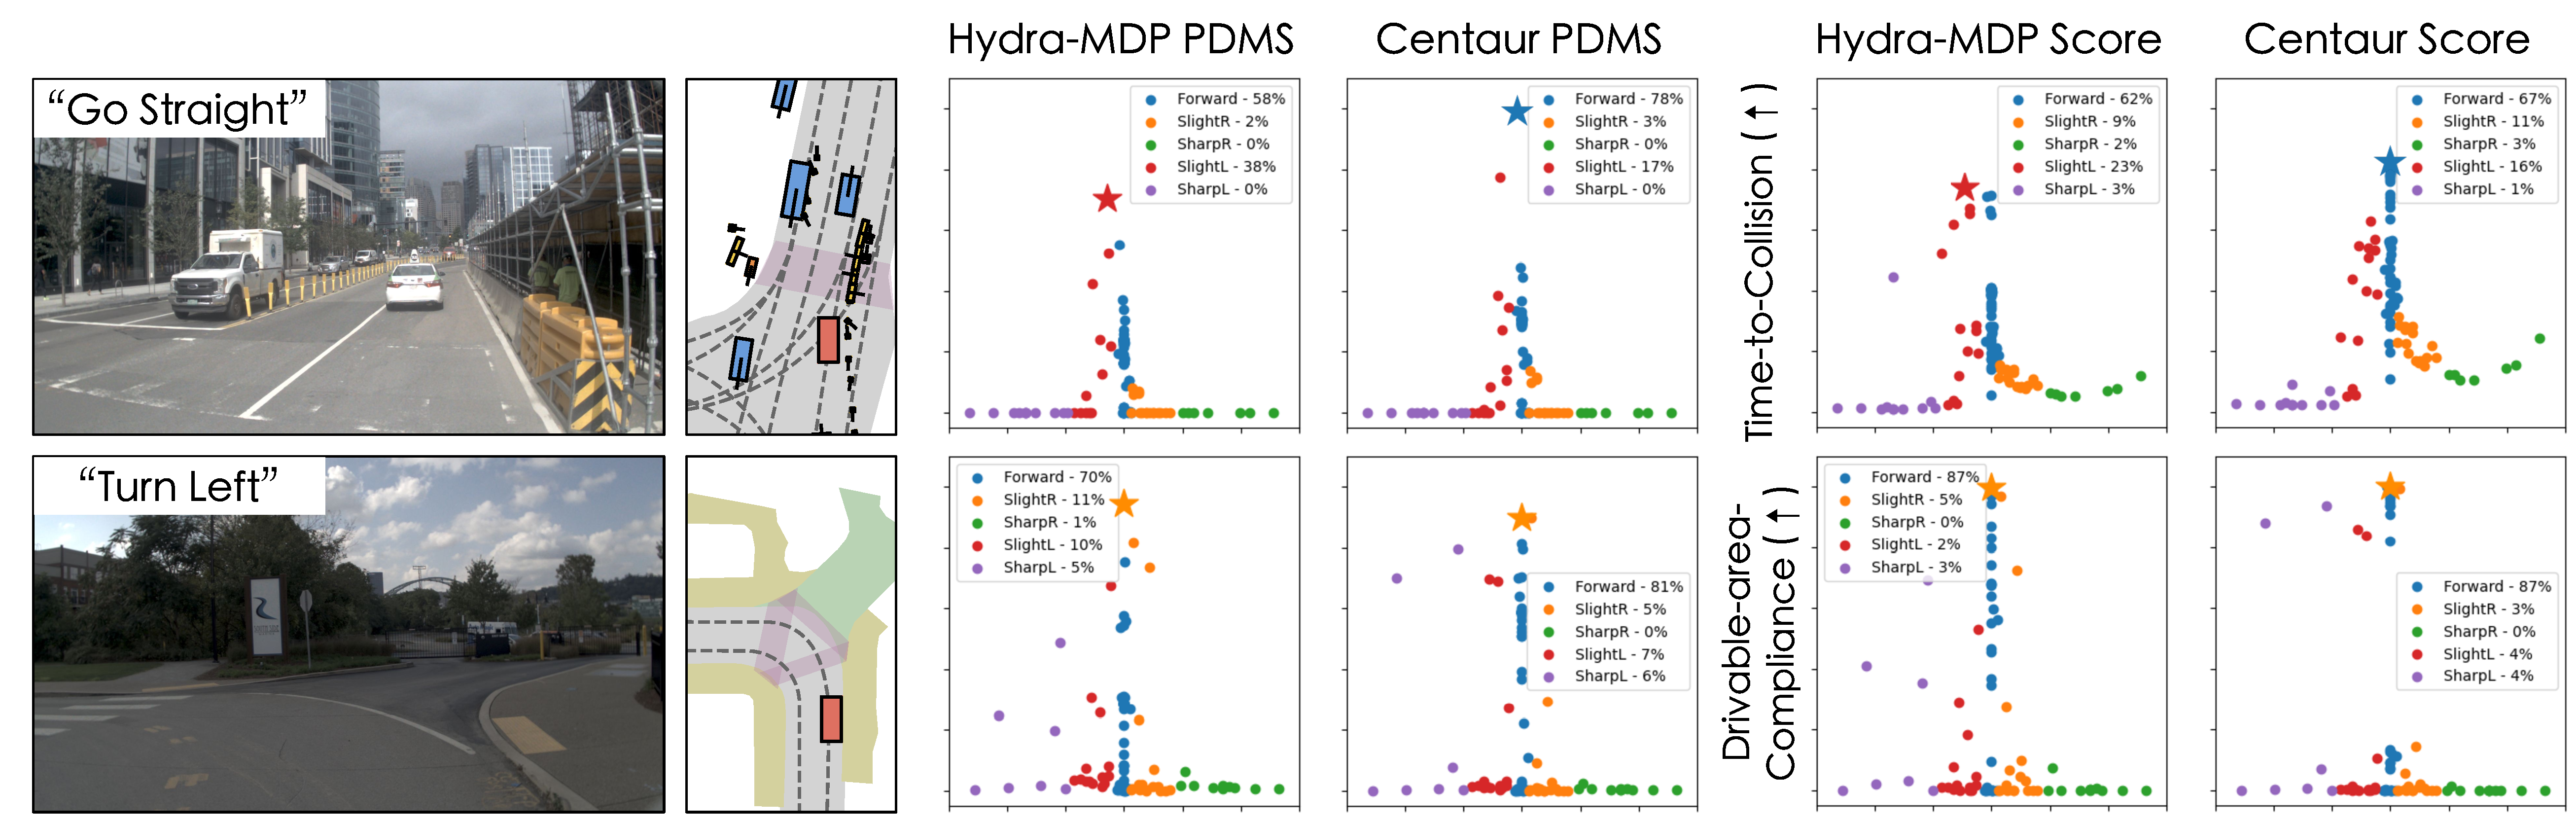
\includegraphics[width=\textwidth]{ch-centaur/images/vis_v7.pdf}
  \caption[Qualitative results of test-time training]{\textbf{Qualitative results.} For each scene, we show the PDMS and a selected sub-score for both Hydra-MDP (before TTT) and Centaur (after TTT), with the highest predicted score marked by $\bigstar$. The x-axis of each plot is the lateral end-point position of the candidate trajectory. \textbf{Top:} TTT helps Centaur, which is uncertain between `Forward' and `Slight Left', to prefer the direction whose cluster members have a higher average score, improving safety. \textbf{Bottom:} A failure case, in which TTT cannot suppress a confident original prediction.}
  \label{centaur:fig:vis}
\end{figure}

The direction clusters also make the score distribution easier to inspect. Fig.~\ref{centaur:fig:vis} visualises two scenarios. In the top row, Hydra-MDP without TTT favours a slight-left trajectory that has a smaller time-to-collision margin; after TTT, Centaur selects a forward trajectory with the better displayed score. In the bottom row, TTT raises the Drivable Area Compliance scores of two `Sharp Left' candidates without making either the top-scoring candidate, so the selected trajectory is unchanged.

\subsection{Generality and Design Choices}\label{centaur:sec:ablations}

\paragraph{Trajectory regression planners.} The source also applies TTT to trajectory regression. Equipping TransFuser~\cite{chitta2023transfuser} with evidential uncertainty (Appendix~\ref{centaur:app:regression}) and using Semantic Entropy changes the reported NAVSIM v1.0 PDMS from 83.4 to 85.7; evidential-uncertainty TTT reports 84.2 (Table~\ref{centaur:tab:navtest_all_supp}). The fallback rows in the same table are retained as source records but not interpreted because they share the aggregation concern identified above.

\paragraph{Test-time optimisation with explicit representations.} Table~\ref{centaur:tab:navtest_all_supp} preserves two NAVSIM v1.0 source comparisons. UniAD's occupancy-based optimisation changes its PDMS from 83.4 to 75.2 and EP from 78.8 to 71.9; adding an explicit 3D occupancy head to PARA-Drive changes its PDMS from 84.0 to 83.6. These observations motivate evaluating alternative adaptation strategies under the same protocol, but they do not show that explicit representations or safety costs are generally harmful.

\paragraph{Combining historical gradients.} Following~\cite{Gao2024fstta}, the historical gradients could alternatively be combined via a singular-value decomposition (SVD) that selects the most useful ones for updating the model. On TransFuser-SE, this variant lowers the PDMS from 85.7 to 83.8 compared with simple averaging (Table~\ref{centaur:tab:navtest_ablation_supp}).

\paragraph{Buffer length.} The number of history frames $F$ has little effect: Hydra-SE obtains 91.4, 91.3, 91.5 and 91.8 PDMS for $F=1$, $2$, $3$ and $4$, respectively (Table~\ref{centaur:tab:navtest_ablation_supp}). Performance increases slightly with longer buffers, with $F=2$ being the lowest, and the consistency across all settings indicates the robustness of the approach.

\paragraph{Image backbone.} With the \mbox{V2-99} backbone, the source reports 90.3 PDMS without TTT and 91.5 with KL-based TTT; the corresponding ViT-L values are 89.9 and 90.9. Fixed-bank fallback values are also reported in Table~\ref{centaur:tab:navtest_ablation_supp}, but are not compared here pending aggregation verification.

\subsection{Computational Cost}\label{centaur:sec:latency}

Table~\ref{centaur:tab:navtest_ablation_supp} reports the amortised latency per frame on \texttt{navtest}, measured on a single NVIDIA A100 GPU. The base Hydra-MDP takes 243.9\,ms, compared with 103.1\,ms for TransFuser, whose efficient ResNet-34 backbone comes at a cost of around 7 PDMS. In the current implementation, the latency of TTT includes the gradient calculation and the model update: with TTT and Semantic Entropy, Hydra-MDP takes 312.5\,ms, and 357.1\,ms with KL Divergence. This overhead could be reduced by computing the gradients in parallel with inference, as described in Section~\ref{centaur:sec:ttt}, or by applying TTT only on frames whose uncertainty exceeds a threshold, which lowers the latency of Hydra-SE to 279.6\,ms at 91.3 PDMS.

%-------------------------------------------------------------------------------
\section{Discussion and Limitations}\label{centaur:sec:discussion}

\paragraph{Self-correction within the evaluated protocol.} The reported TTT rows improve safety-related sub-scores while nearly maintaining progress (EP changes from 86.5 to 85.9 on \texttt{navtest}). The fixed-bank fallback rows instead show higher NC, DAC and TTC with much lower EP, but their aggregate columns require the record check in Section~\ref{centaur:sec:results}. UniAD's source-reported cost-function optimisation also reduces EP and PDMS (Table~\ref{centaur:tab:navtest_all_supp}). These restricted comparisons do not establish that TTT replaces general safety filters; they show that an update using the planner's own uncertainty can improve the reported NAVSIM scores without new labels or a scene-dependent test-time cost. On \texttt{navsafe}, Centaur has the highest score in seven of ten categories but regresses on yielding from 71.6 to 59.3. The unresolved Overall aggregation and the model-dependent split selection preclude a verified aggregate tail-improvement claim.

\paragraph{How much of the gain is due to Cluster Entropy?} The headline improvement from 90.3 to 92.6 PDMS comes from a single training run evaluated with NAVSIM v1.0 (Table~\ref{centaur:tab:navtest_ablation}). Over three seeds on the NAVSIM v1.1 leaderboard, Centaur leads Hydra-SE, its own Semantic Entropy variant, by only 0.23 PDMS (92.10 $\pm$ 0.33 \vs 91.87 $\pm$ 0.19; Table~\ref{centaur:tab:navtest_all}), less than Centaur's own standard deviation across seeds, and no significance test was run. Moreover, all four uncertainty measures used for TTT in Table~\ref{centaur:tab:navtest_ablation}, three entropies and a KL divergence, improve Hydra-MDP by between 1.2 PDMS (KL Divergence) and 2.3 PDMS (Cluster Entropy). This suggests that much of the benefit comes from minimising an entropy-style uncertainty at test time in general, rather than from the specific form of Cluster Entropy, whose distinctive advantage is better supported for interpretability (Section~\ref{centaur:sec:qualitative}) than for accuracy.

\paragraph{Interpretability and failure detection.} Because its five clusters correspond to driving directions, Cluster Entropy lets a reader inspect which alternatives receive score mass (Figs.~\ref{centaur:fig:teaser} and~\ref{centaur:fig:vis}); this is not evidence of a faithful explanation of the decision. At one threshold, it also has the highest reported TPR among the compared measures for flagging source-defined failure frames (62.8\%, Table~\ref{centaur:tab:fail_class}). This evidence is limited: the exact failure predicate is unavailable, its accuracy of 73.6\% is below the 84.4\% Select None baseline, and AUROC and AUPRC were not reported.

\paragraph{Limitations.} As an early attempt, Centaur shows promising performance, but it has several limitations. First, it is evaluated only in the non-reactive simulation of NAVSIM v1, which scores planned trajectories with principled, rule-based metrics but does not let other road users react; it has not been tested in reactive closed-loop simulation or on a vehicle. NAVSIM has since been extended to version~2, which is based on pseudo-simulation~\cite{cao2025pseudo}; Centaur has not been evaluated under this protocol. Extending it to a closed-loop setting with an affordable inference budget is a promising direction to explore. Second, test-time compute is quite limited in autonomous driving, which is an efficiency-sensitive task. The measured latency of TTT currently includes the gradient calculation (Section~\ref{centaur:sec:latency}), and it is worth exploring ways of unifying TTT and model inference to minimise the compute overhead. Third, because the objective only rewards confidence, TTT can correct outlier scores but cannot suppress a confident original prediction, as the failure case in Fig.~\ref{centaur:fig:vis} shows. Relatedly, Centaur is highest in seven displayed \texttt{navsafe} categories but not in every category. On YLD it regresses from the 71.6 of Hydra-MDP to 59.3, below both Hydra-SE (84.6) and TransFuser (61.6), a regression that matters for pedestrians and other vulnerable road users. It also trails Hydra-SE (64.4) and LTF (62.8) on BWTH (60.2), and LTF on YLLT (65.0 \vs 70.2). On \texttt{navtest}, its ego progress is slightly lower than that of Hydra-MDP (85.9 \vs 86.5). Fourth, \texttt{navsafe} is small: five of its ten categories contain between 5 and 12 frames, so per-category scores should be interpreted with care. It was selected partly by Hydra-MDP performance, no confidence intervals are reported, and the Overall score cannot be recomputed from the published category scores. Finally, the source records needed to pin the local scorer, failure predicate and fixed-bank aggregation are absent from the thesis repository. These gaps are marked for recovery before submission.

%-------------------------------------------------------------------------------
\section{Chapter Summary}\label{centaur:sec:summary}

This chapter addressed RQ3a: whether a deployed end-to-end driving policy can improve under shift through a test-time update that queries no new expert labels and evaluates no scene-dependent explicit safety cost. Centaur updates the score decoder by reducing Cluster Entropy, a direction-cluster score-mass measure derived from sampled candidate trajectories. The candidate bank and five direction rules are fixed design choices, and unequal cluster sizes can affect the entropy. The exact update/reset semantics still require verification against the implementation. The chapter also releases \texttt{navsafe}, 229 \texttt{navtest} frames in ten NHTSA-inspired categories, as a model-selected diagnostic stress set rather than an unbiased estimate of natural safety-event performance.

In a single training run on \texttt{navtest} with NAVSIM v1.0, Centaur raises the PDMS of Hydra-MDP from 90.3 to 92.6, with the largest sub-score gain in time-to-collision (from 93.9 to 98.0) and a slight loss in ego progress (from 86.5 to 85.9). The fixed-bank fallback records show much lower progress, but their aggregation requires verification. With a mean PDMS of 92.10 $\pm$ 0.33 over three seeds, Centaur ranked first among three-seed entries on the official NAVSIM v1.1 \texttt{navtest} leaderboard at the paper's submission in March 2025. Its lead over Hydra-SE is only 0.23 PDMS, and every tested uncertainty objective improves Hydra-MDP by 1.2--2.3 PDMS. At one selected threshold, Cluster Entropy has the highest reported TPR (62.8\%) among the compared measures, but its accuracy (73.6\%) is below Select None (84.4\%). On \texttt{navsafe}, Centaur leads seven of ten displayed categories but regresses on yielding from 71.6 to 59.3; the source Overall aggregation is unresolved and is therefore not a thesis conclusion. TTT also transfers to TransFuser (+2.3 reported PDMS with Semantic Entropy), while UniAD's source-reported cost optimisation lowers its PDMS from 83.4 to 75.2. The main limitations are non-reactive simulation, added test-time compute, the small margin over other uncertainty objectives, model-dependent stress-set selection, unresolved source records and the inability of entropy minimisation to overturn a confident wrong prediction.

Driving policies thus benefit from test-time self-correction, at least in non-reactive simulation: a planner that can measure its own uncertainty can turn it into a training signal after deployment. In robot manipulation, however, the gap between training and deployment is even wider. Human demonstrations are inconsistent, data and compute are limited, and hardware behaves differently at deployment than during data collection. Chapter~\ref{ch:kai0} tackles this setting.
